\chapter{Backend}
\label{backend}

\section{Architektur}
Das Backend besteht aus zwei logisch und derzeit auch physisch getrennten Servern. 
Der Webserver liefert die \gls{WebApp} aus und ist auch der einzige Kommunikationspartner für das Frontend. Dies ist zum einen eine architektonische, zum anderen eine technische Entscheidung.

\begin{itemize}
\item Das Frontend muss sich nicht darum kümmern woher es welchen Dienst bezieht
\item Die Same-Origin-Policy\cite{sop} einiger Server lässt keine direkte Kommunikation zwischen \emph{fremdem} JavaScript und dem Server zu
\end{itemize}

Der Webserver ist somit der Dreh- und Angelpunkt der Applikation, jegliche Informationen von und zum Frontend durchläuft diese zentrale Komponente.

Da der 


\section{REST-Schnittstellen}



\todo[inline]{Slim}

\section{Kommunikation/Transaktionen}

\section{OAuth}
\label{oauth}

\begin{figure}[H]
\subfigure{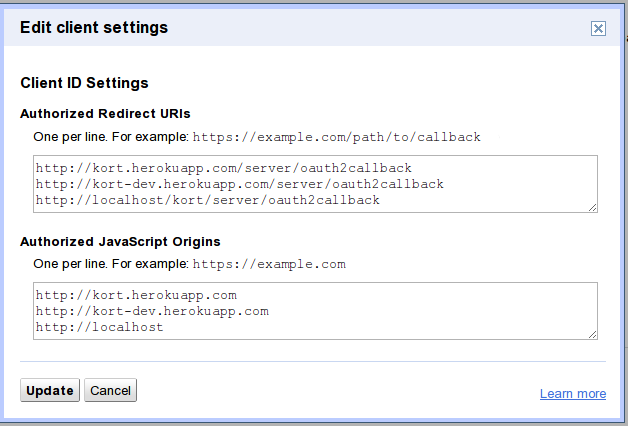
\includegraphics[scale=0.5]{images/backend/oauth-google-settings}}
\caption{OAuth Einstellungen}
\end{figure}

Der erfolgreiche Login wird direkt in der Session des Benutzers gespeichert.
Auf die entsprechenden Werte wird dann bei sicherheits-kritischen